%!TEX program = lualatex
% ^use lualatex for best compatibility

\documentclass[
	ngerman, % TODO: Or 'english' if you write in English
	ruledheaders=section,%Ebene bis zu der die Überschriften mit Linien abgetrennt werden, vgl. DEMO-TUDaPub
	class=report,%Basisdokumentenklasse. Wählt die Korrespondierende KOMA-Script Klasse
	thesis={type=master},%Dokumententyp Thesis, für Dissertationen siehe die Demo-Datei DEMO-TUDaPhd
	accentcolor=1b,%Auswahl der Akzentfarbe
	custommargins=false,% Ränder werden mithilfe von typearea automatisch berechnet
	marginpar=false,% Kopfzeile und Fußzeile erstrecken sich nicht über die Randnotizspalte
	BCOR=12mm,%Bindekorrektur, falls notwendig
	twoside,%größerer Rand ist abwechselnd rechts und links
	open=right, %TODO: Kann bei rein digitalen Abgaben entfernt werden; neue Kapitel starten immer auf der rechten Seite (ggf. wird also eine leere Seite eingefügt)
	parskip=half-,%Absatzkennzeichnung durch Abstand vgl. KOMA-Sript
	fontsize=11pt,%Basisschriftgröße laut Corporate Design ist mit 9pt häufig zu klein
	IMRAD=false,%Abschalten von IMRAD-Warnings wegen fehlender Labels
	bibliography=totoc,%Literaturverzeichnis im Inhaltsverzeichnis
	pdfa=true,
	%	toc=flat,%https://github.com/tudace/tuda_latex_templates/issues/326#issuecomment-889819154
	numbers=noenddot, % Remove dots at the end of all numbers; https://tex.stackexchange.com/a/40045
]{tudapub}

% Der folgende Block ist nur bei pdfTeX auf Versionen vor April 2018 notwendig
\usepackage{iftex}
\ifPDFTeX
\usepackage[utf8]{inputenc}%kompatibilität mit TeX Versionen vor April 2018
\fi

%%%%%%%%%%%%%%%%%%%
%Sprachanpassung und Verbesserte Trennregeln
%%%%%%%%%%%%%%%%%%%
\usepackage[english, main=ngerman]{babel} % TODO: Or 'main=english' if you write in English
\usepackage{microtype}

%%%%%%%%%%%%%%%%%%%
%Beschriftung von Tabellen, Skizzen, Listings etc.
%%%%%%%%%%%%%%%%%%%
\usepackage{caption}
\captionsetup{justification=centering}

%Tabellen
%%%%%%%%%%%%%%%%%%%
%\usepackage{array}     % Basispaket für Tabellenkonfiguration, wird von den folgenden automatisch geladen
\usepackage{tabularx}  % Tabellen, die sich automatisch der Breite anpassen
%\usepackage{longtable} % Mehrseitige Tabellen
%\usepackage{xltabular} % Mehrseitige Tabellen mit anpassarer Breite
\usepackage{booktabs}   % Verbesserte Möglichkeiten für Tabellenlayout über horizontale Linien

%%%%%%%%%%%%%%%%%%%
%Paketvorschläge Mathematik
%%%%%%%%%%%%%%%%%%%
\usepackage{mathtools}  % erweiterte Fassung von amsmath
\usepackage{amssymb}    % erweiterter Zeichensatz
% SI Basiseinheiten mit bits und Bytes
\usepackage[binary-units=true]{siunitx}

%%%%%%%%%%%%%%%%%%%
% Code-Listings und Illustrationen
%%%%%%%%%%%%%%%%%%%
\usepackage{listings}   % ermöglicht es Quell-code schön darzustellen
\usepackage{graphicx}
%%%%%%%%%%%%%%%%%%%

%%%%%%%%%%%%%%%%%%%
%Referenzen und Links
%%%%%%%%%%%%%%%%%%%
\usepackage{hyperref} % erzeugt aus Referenzen und Web-Adressen Hyperlinks zum Springen im Dokument oder dem Öffnen einer Webseite.
% https://tex.stackexchange.com/questions/195976/change-the-output-format-of-cref-from-table-to-table-and-from-eq-to-equation
\usepackage[noabbrev]{cleveref} % automatisches Voranstellen des Referenztyps (z.B. Kapitel)
%%%%%%%%%%%%%%%%%%%

%%%%%%%%%%%%%%%%%%%
%Umgebungen für Beispiele und Definitionen
%%%%%%%%%%%%%%%%%%%
\usepackage{amsthm}
\newtheorem{definition}{Definition}[chapter]
\newtheorem{theorem}{Theorem}[chapter]
\newtheorem{lemma}{Lemma}[chapter]
\newtheorem{corollary}{Korollar}[chapter]
\newtheorem{proposition}{Propostion}[chapter]
\newtheorem{example}{Beispiel}[chapter]


\usepackage{lipsum} % TODO: Blindext im Beispiel erzeugen (kann entfernt werden)


% Deutsche Anführungszeichen
% TODO: You have to adapt this if you write in English and you use this command
\newcommand{\enquot}[1]{“{}#1”{}}

% Inline Aufzählungen
\usepackage{paralist}

% Aufzählungen mit angepassten items
\usepackage[inline]{enumitem}

% Colorbox
\usepackage{color}

% Abkürzungsverzeichnis
\usepackage{acronym}

% tikz
% TODO: Tikz Pakete einbinden, falls tikz benötigt wird
%\usepackage{tikz}
%\usepackage{pdfpages}
%\usepackage{pgfplotstable}
%\usepackage{pgfplots}
%% https://github.com/xuyuan/pgf-umlcd/issues/17
%%\usepackage{tikz-uml}
%\let\attribute\relax
%\usepackage[simplified]{pgf-umlcd}
%\usetikzlibrary{shapes,arrows,positioning,fit,calc}
%\usetikzlibrary{shapes.geometric}
%\usepgfplotslibrary{units}
%\pgfplotsset{compat = 1.3}
%\usepackage{makecell}

% Circle around symbols
% TODO: Einkommentieren, falls Kreise um Symbole im Text benötigt werden sollten
%\newcommand*\circled[1]{\tikz[baseline=(char.base)]{
%		\node[shape=circle,draw,inner sep=1pt,minimum height=1em] (char) {#1};}}

% centering captions
\usepackage[justification=centering,labelfont=bf]{caption}

% Subcaptions
\usepackage{subcaption}

% custom texttt
\newcommand{\texttts}[1]{\texttt{\small #1}}
\newcommand{\textttss}[1]{\texttt{\scriptsize #1}}

% Rotate figures
\usepackage{rotating}

% Temporary fix for figure placement
\usepackage[section]{placeins}
\usepackage{float}

% TODO: Wenn du CSV-Dateien laden möchtest, könnte dieses Paket hilfreich sein.
% Load CSV files
%\usepackage{csvsimple}

% Break URLs
\usepackage{url}
\def\UrlBreaks{\do\/\do-}

% Add type for equations in floats
% https://stackoverflow.com/questions/149479/adding-a-caption-to-an-equation-in-latex
\DeclareCaptionType{equ}[][]

% Fix LOF and LOT spacing errors
% https://tex.stackexchange.com/a/187202
% TODO: Falls Platzprobleme in den automatischen Listen (figures, tables) passieren, könnte das hilfreich sein:
%\usepackage[titles]{tocloft}
%\cftsetindents{figure}{0em}{2.5em}
%\cftsetindents{table}{0em}{2.5em}

% Fix subfigure referece using \cref
% https://tex.stackexchange.com/a/180382
\captionsetup[subfigure]{subrefformat=simple,labelformat=simple}
\renewcommand\thesubfigure{(\alph{subfigure})}

% Diagonal fractions
% https://tex.stackexchange.com/questions/3372/how-do-i-typeset-arbitrary-fractions-like-the-standard-symbol-for-5-%C2%BD
% TODO: Einkommentieren, falls diagonale Brüche gewünscht werden
%\usepackage{xfrac}


\begin{document}

\frontmatter

\Metadata{
	title=Hier steht der mehrzeilige Titel der Thesis,
	author=Jane Doe
}

\title{Hier steht der mehrzeilige Titel der Thesis}
\subtitle{This is the English Title of the Thesis} %oder der deutsche Titel, falls Thesis in englisch geschrieben wird
\author[J. Doe]{Jane Doe}%optionales Argument ist die Signatur
% \studentID{12345678}%Benutzung, falls gewünscht
\reviewer{Prof.~Dr.~rer.~nat.~Andy Schürr \and Erika Mustermann,~M.\,Sc.}%Gutachter
% TODO: Nach Anmeldegespräch Nummer bei Betreuer erfragen und hier anpassen!
\titleaddendum{ES-M-123}

%Diese Felder werden untereinander auf der Titelseite platziert. 
\department{etit} % Das Kürzel wird automatisch ersetzt und als Studienfach gewählt, siehe Liste der Kürzel im Dokument.
\group{Fachgebiet Echtzeitsysteme}
% TODO: Or 'Real-Time Systems Lab' if you write in English
%\group{Real-Time Systems Lab}

\submissiondate{\today}
\examdate{\today}

% \tuprints{urn=1234,printid=12345}
% \dedication{Für alle, die \TeX{} nutzen.}

\maketitle

% TODO
\affidavit % benutzen, wenn die Thesis gedruckt und digital eingereicht wird
% \affidavit[digital] % benutzen, wenn die Thesis ausschließlich digital eingereicht wird

\section*{Guidelines für Seminararbeiten und Thesen}

Eingebettet in diese Vorlage findest du eine kurze Anleitung, die dir hilft deinen (ersten) wissenschaftlichen Text zu verfassen.
Dabei kann es sich um ein Paper im Zuge einer Seminararbeit oder auch deine erste Thesis handeln.
Weshalb wir diese Guidelines in Text gegossen haben, ist der einfache Fakt, dass fast jeder zu Anfang dieselben Fehler macht.
Deshalb soll dir dieses Dokument als kleines Nachschlagwerk dienen.
Denke dabei daran diese Teile für die finale Abgabe aus deiner Vorlage zu löschen!

Wichtig: Diese Auflistung erhebt keinen Anspruch auf Vollständigkeit und falls etwas unklar oder unerwähnt bleibt, solltest du dich immer zeitnah an deinen Betreuer wenden.
Auch wären wir über Feedback froh, damit nachfolgende Studenten von dieser Sammlung noch mehr profitieren können. (kontakt(at)es.tu-darmstadt.de) 

Natürlich solltest du auch immer die Richtlinien deines Fachbereichs beachten:
\begin{itemize}
	\item \href{https://www.etit.tu-darmstadt.de/media/etit/studium_1/dokumente_4/richtlinien/richtlinienabschlussarbeiten.pdf}{\color{blue}{Fachbereich Elektrotechnik und Informationstechnik}}
	\item \href{https://www.informatik.tu-darmstadt.de/studium_fb20/im_studium/studienbuero/abschlussarbeiten_fb20/index.de.jsp}{\color{blue}{Fachbereich Informatik}}
\end{itemize}

\section*{Strukturierung}
Fast jede Ausarbeitung ob Paper oder Thesis folgt einer klaren Struktur. 
Es ist an gewissen Stellen sicherlich kein Fehler davon abzuweichen und es kommt auf die Community an, in der man publiziert. 
Allgemein gesprochen gibt es jedoch „konventionsgemäße“ Überschriften:
\begin{itemize}
	\item Abstract / Zusammenfassung
	\item Introduction / Einleitung
	\item Background / Grundlagen
	\item Contribution / Eigener Beitrag
	\item Related Work / Verwandte Arbeiten
	\item Conclusion (= Summary + Outlook) / Abschluss (= Zusammenfassung + Ausblick)
\end{itemize}

Im Folgenden findest du zu jedem dieser Unterpunkte ein paar Erläuterungen.
Lese sie alle durch und verinnerliche sie, bevor du mit dem Aufschreiben anfängst.
Unsere Erfahrung zeigt, dass dies dir viel Arbeit sparen kann!

%!TEX root = ../thesis-main.tex

\begin{abstract}[ngerman]
Dies ist eine High-Level Beschreibung deiner gesamten Arbeit, die vor allem kurz und prägnant sein soll. 
Aus diesem Grund ist sie für gewöhnlich eine der letzten Passagen, die man verfasst, wenn der Großteil der Arbeit bereits weit fortgeschritten ist. 
Prinzipiell geht es darum, das Problem möglichst kompakt zu präsentieren (gegebenenfalls auch zu motivieren) und danach ebenso kompakt seine Lösung zu skizieren.
\\
\\
Die Zusammenfassung wird hier auf Deutsch verfasst. 
\end{abstract}
\acresetall
%!TEX root = ../thesis-main.tex

\begin{abstract}[english]
Hier steht die englische Zusammenfassung deiner Arbeit.
\end{abstract}

% Reset all acronyms after the abstracts
\acresetall

\tableofcontents
\clearpage
\cleardoublepage

% TODO: Das Abkürzungsverzeichnis ist optional! Hier einkommentieren, falls es benutzt werden soll.
%% Abkürzungsverzeichnis
%% Abkürzungsverzeichnis
% TODO: Das Abkürzungsverzeichnis ist optional!

% TODO: Change to 'List of Abbreviations' if you write in English
\section*{Abkürzungsverzeichnis}
\label{sec:list-of-abbreviations}
%\addcontentsline{toc}{chapter}{\protect\numberline{}List of Abbreviations}

% TODO: Sort after everything is included
\begin{acronym}[AAAAAA] % optional argument formats the horizontal space
	\acro{CPU}[CPU]{Central Processing Unit}
	\acro{EMF}[EMF]{Eclipse Modeling Framework}
	\acro{GT}[GT]{Graph Transformation}
	\acro{ILP}[ILP]{Integer Linear Programming}
	\acro{MDSE}[MDSE]{Model-driven Software Engineering}
	\acro{MOF}[MOF]{Meta Object Facility}
	\acro{MT}[MT]{Model Transformation}
	\acro{NAC}{Negative Application Condition}
	\acro{OMG}[OMG]{Object Management Group}
	\acro{SOS1}{Special Ordered Set 1}
	\acro{VM}[VM]{Virtual Machine}
	\newacroplural{VM}[VMs]{Virtual Machines}
\end{acronym}
% Ende des Abkürzungsverzeichnisses

%\clearpage
%\cleardoublepage

% Auflistung Abbildungen
% https://tex.stackexchange.com/questions/784/how-to-change-the-line-spacing-in-my-list-of-figures
\newcommand*{\noaddvspace}{\renewcommand*{\addvspace}[1]{}}
\addtocontents{lof}{\protect\noaddvspace}
\listoffigures
\label{sec:list-of-figures}
%\addcontentsline{toc}{chapter}{\protect\numberline{}List of Figures}
\cleardoublepage
\clearpage

% Auflistung Tabellen
\addtocontents{lot}{\protect\noaddvspace}
\listoftables
\label{sec:list-of-tables}
%\addcontentsline{toc}{chapter}{\protect\numberline{}List of Tables}
\cleardoublepage
\clearpage

\mainmatter

%!TEX root = ../thesis-main.tex

\chapter{Einleitung}\label{chapter:introduction}

Ähnlich wie im Abstract soll hier das Problem definiert werden und die Lösung angedeutet werden.
Der Unterschied liegt vor allem in der Ausführlichkeit mit der dies geschieht. 
Das Wichtigste in der Introduction ist die Motivation des Ansatzes: 
\begin{itemize}
	\item \emph{Was ist das Problem?}
	\item \emph{Warum gibt es überhaupt das Problem? }
	\item \emph{Warum will man dies lösen bzw. wieso ist das Problem relevant? }
	\item \emph{Warum ist dein Ansatz notwendig und was soll er leisten (abstrakt)?}
\end{itemize}
In der Forschung gibt es zum Beispiel das CARS-Konzept\footnote{https://libguides.usc.edu/writingguide/CARS}: "Creating a Research Space".
Man geht dabei von einem sehr wichtigen Problem aus und beschreibt, warum es eine ungelöste Nische gibt, die man mit diesem Paper/Arbeit genau füllt.

Es hilft hierbei auch Beispiele zu beschreiben, wenn möglich aus der echten Welt, um dem Leser ein bildhaftes Verständnis der Problematik zu vermitteln.
Am Ende der Introduction sollte die Struktur der restlichen Arbeit eingeführt werden, mit jeweils höchstens einem Satz für jedes Kapitel.

\textbf{Faustregel}: max 10\% Introduction, max 10\% Conclusion


\section{Sonstiges}
\textbf{WICHTIG:} Falls die Thesis ausschließlich digital eingereicht wird (also ohne zusätzliche gedruckte Version), muss in der Datei \texttt{thesis-main.tex} der Befehl \texttt{\textbackslash affidavit} durch \texttt{\textbackslash affidavit[digital]} ersetzt werden.
Dadurch wird die eidesstattliche Erklärung entsprechend angepasst.

Diese Vorlage ist für doppelseitigen Druck eingestellt.
Es ist voreingestellt, dass eine PDF/A-Datei erzeugt wird.
Die beste Kompatibilität hierfür bietet Lua\LaTeX.
Bei anderen Compilern kann dies entsprechend der Informationen in DEMO-TUDaPub zu Problemen führen.
In diesem Fall sollte entweder der Compiler gewechselt oder \texttt{pdfa=false} aktiviert werden.
Dies ist eine Referenz zu Kapitel~\ref{chapter:background}.
Dies ist eine Referenz zu Abschnitt~\ref{sect:dummy-section}.
Dies ist eine Referenz auf eine Quelle~\cite{Luthmann2017}.
Dies ist eine Referenz auf zwei Quellen~\cite{Luthmann2019,Ruland2018}.
Dies ist eine Referenz auf eine Onlinequelle~\cite{parallel-computing}.
Bei Zitationen von Onlinequellen gibt es ein paar Dinge, die beachtet werden müssen:
\begin{itemize}
	\item Zur Literaturverwaltung wird BibTeX verwendet, d.h. es gibt \textbf{keine} \texttt{@online} Typen in der Bibliographie-Datei. Stattdessen verwenden wir \texttt{@misc} und bauen die korrekte Zitierweise per Hand.
	\item Je nachdem, ob in Deutsch oder in Englisch geschrieben wird, muss der String \enquot{Letzter Zugriff:} angepasst werden zu \enquot{Last accessed:}.
	\item Bitte verwende bei den Datumsangaben ausschließlich das ISO-Format (\texttt{\$jahr-\$monat-\$tag}), beispielsweise \texttt{2024-05-07} für den 07. Mai 2024.
\end{itemize}



\section{Überschrift eines Abschnitts}\label{sect:dummy-section}

%\lipsum

{\Huge Hier} {\huge steht} {\LARGE ein} {\Large kurzer} {\large Satz} {\normalsize mit} {\small immer} {\footnotesize kleiner} {\scriptsize werdender} {\tiny Schriftgröße}.
%!TEX root = ../thesis-main.tex

\chapter{Grundlagen}\label{chapter:background}
In diesem Kapitel müssen die Grundlagen präsentiert und eingeführt werden, die ein Leser benötigt, um deinen Text zu verstehen.
Man sollte sich hierbei vornehmen, die Grundlagen so einzuführen, dass auch ein fachfremder Leser diese verstehen kann.
Hierzu gehören Theorien, Frameworks und andere Arbeiten, die essentiell sind, um die weiteren Kapitel verstehen zu können. 
Damit das gut klappt, sollte ein gutes Beispiel gewählt werden, welches sich möglichst auch durch den Rest der Arbeit zieht.
Somit werden die Ausführungen nachvollziehbarer und man kann einzelne Schritte besser in Bezug zueinander setzen.

Darüber hinaus sollten die einzelnen diskutierten Themen so angelegt werden, dass möglichst keine Vorwärtsreferenzen entstehen (siehe Schreibstil). 
Auch solltest du einen guten Kompromiss zwischen einer zu kurzen und einer zu langen Erläuterung finden (siehe Schreibstil).



\section{Illustratives Beispiel}\label{sect:motivating-examples}
Illustrationen, Tabellen und andere Elemente helfen dabei einen Sachverhalt oder auch Ergebnisse besser darzustellen. Damit diese Helfer auch einen Bezug zum Text haben, sollten sie aus dem Fließtext heraus immer mindestens einmal \underline{sinnvoll} referenziert worden sein.
In Latex kann man so etwas recht komfortabel mit \lstinline|\ref(<label>)| bewerkstelligen. Damit lässt sich später im PDF-Dokument mit einem einfachen Klick zu den Referenzen springen, was den Bezug zum Text verbessert und letztlich das Verständnis fördert.\\
Beispiel: Dies ist eine Referenz zu Kapitel~\ref{chapter:introduction}.\\ 
Um mögliche Inkonsistenzen beim Referenzieren von Kapiteln, Skizzen, Tabellen o.Ä. zu vermeiden, empfehlen wir die Verwendung des Paketes Cleverref. Damit werden automatisch Bezeichner wie \glqq Kapitel\grqq{} oder \glqq Section\grqq{} in der korrekten Sprache vor die Referenz gestellt.\\
Beispiel: Dies eine weitere Referenz zu \cref{chapter:introduction}.\\
Illustrationen (\cref{fig:some-figure}), andere Elemente wie z.B. Tabellen (\cref{table:some-table}), Definitionen (\cref{def:dummy-def}) oder Beispiele (\cref{example:dummy-example}) lassen sich genauso einfach referenzieren.
%\lipsum[2-3]

\begin{figure}
    \centering
    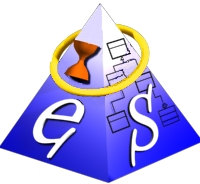
\includegraphics[width=.3\linewidth]{figures/es_logo_gross.jpg}
    \caption{Dies ist eine Beispiel-Abbildung, die das Logo des Fachgebiets zeigt.}\label{fig:some-figure}
\end{figure}

\begin{figure}
    \centering
    % Erste Abbildung
    \begin{subfigure}[b]{0.48\textwidth}
	\centering
        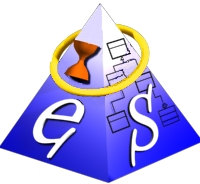
\includegraphics[width=.4\linewidth]{figures/es_logo_gross.jpg}
        \subcaption{Subfigure Bild Nr.\,1}
    \end{subfigure}
    % Zweite Abbildung
    \begin{subfigure}[b]{0.48\textwidth}
        \centering
        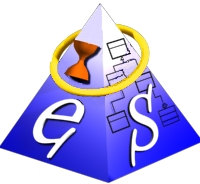
\includegraphics[width=.4\linewidth]{figures/es_logo_gross.jpg}
        \subcaption{Subfigure Bild Nr.\,2}
    \end{subfigure}
    \caption{Es ist auch möglich Abbildungen mit Unterabbildungen zu erstellen.}\label{fig:some-sub-figure}
\end{figure}

%\lipsum[4-5]

\begin{definition}[Timed Automaton]\label{def:dummy-def}
Ein \emph{Timed Automaton (TA)} ist ein Tupel $\mathcal{A}=(L,\ell_0,\Sigma,C,I,E)$, bei dem
\begin{itemize}
	\item $L$ eine endliche Menge von \emph{Orten} ist,
	\item $\ell_0\in L$ der \emph{Startort} ist,
	\item $\Sigma$ eine endliche Menge von \emph{Aktionen} mit $L\cap\Sigma=\emptyset$ ist,
	\item $C$ eine endliche Menge von \emph{Uhren} über $\mathbb{T}_C$ mit $C\cap(L\cup\Sigma)=\emptyset$ ist,
	\item $I:L\rightarrow\mathcal{B}(C)$ eine Funktion ist, die Orten \emph{Invarianten} zuweist, und
	\item $E\subseteq L\times\mathcal{B}(C)\times\Sigma\times 2^{C}\times L$ eine endliche Relation ist, die \emph{Kanten} definiert.
\end{itemize}
\end{definition}

%\lipsum[8]

\paragraph{Ein Paragraph}
\lipsum[9]

\begin{example}[Ein Beispiel]\label{example:dummy-example}
\lipsum[5-6]
\end{example}

\begin{table}[tp]
    \centering
    \caption{Dies ist die Beschriftung einer Tabelle.}\label{table:some-table}
    %!TEX root = ../thesis-main.tex

\begin{tabular}{ccccc}
\toprule
Spalte 1 & Spalte 2 & Spalte 3 & Spalte 4 & Spalte 5 \\ \midrule
0 & 8 & 15 & a & b \\
42 & 1 & 1 & c & d \\
1 & 1 & 2 & 3 & 5 \\
\bottomrule
\end{tabular}
\end{table}

%\lipsum[3]

\begin{theorem}[Theorem mit einer Formel]\label{theorem:dummy-theorem}
Dies ist ein Theorem mit der Formel
\begin{equation}
\label{eq:equation1}
\sum_{k=1}^n k=\frac{n(n+1)}{2}=\frac{n^2+n}{2}
\end{equation}
gefolgt von etwas mehr Text, einer Gleichung
$$\sqrt{9}=\pm3\text{ und }2\alpha=4\Rightarrow\alpha=2$$
und noch mehr Text und einer letzten einzeiligen Gleichung \(C = B \log_2 \left(1 + \frac{S}{N} \right) \).
\end{theorem}

\begin{proof}
Dies ist der Beweis von \cref{theorem:dummy-theorem} mit \cref{eq:equation1}.
\end{proof}


Auch Listings von beispielsweise Python-Code lassen sich erstellen und referenzieren
(siehe~\cref{lst:some-listing}).
\begin{lstlisting}[language=Python, caption=Python Listing, label=lst:some-listing]
import random
    
def get_grade(thesis):
    return random.randrange(1,6)
\end{lstlisting}


\section{Inline Code und/oder Begriffe aus Abbildungen}\label{sect-inline-code}

Um im Fließtext auf Code oder Begriffe (wie z.\,B. Klassennamen) aus Diagrammen zu referenzieren, bietet sich
\texttt{\textbackslash\-texttt\{inhalt\}}
an.
Diese Audrücke werden zu \texttt{inhalt} gerendert.

Eine Schwierigkeit dabei könnte sein, dass die String in diesen Fällen nicht immer automatisch oder korrekt umgebrochen werden.
Dafür ist wird in diesem Dokument das Paket \texttt{hyphenat} geladen.
Sollte es einmal Probleme geben, so können LaTeX immer durch \texttt{\textbackslash-} zwischen Silben Hinweise gegeben werden, wie ein Wort zu brechen ist.
Beispiel: \texttt{\textbackslash\-texttt\{langer\textbackslash-Inhalt\textbackslash-Der\textbackslash-Nicht\textbackslash-Umbricht\}}

\section{Akronyme}\label{acronyms}

% Trigger acronyms
Dieser Satz steht hier nur drin, um ein Akronym zu triggern: \ac{VM} und nun noch einmal \ac{VM}.

%!TEX root = ../thesis-main.tex

\chapter{Implementierung}\label{chapter:implementation}

Hier wird der eigentliche eigene Beitrag (engl. Contribution) vorgestellt. 
Dies ist für gewöhnlich der Teil an dem man weniger Probleme hat, weil man z.B. durch das Implementieren genau weiß, was man getan hat und diese Dinge auch eine gewisse Ordnung im Kopf haben (Erst habe ich das gemacht, dann das, dann ...).

Wichtig ist hier zu vermeiden Dinge unter den Tisch fallen zu lassen, die einem trivial vorkommen und deshalb unerwähnt bleiben. 
Dem Leser sind diese Dinge womöglich nicht ganz so klar. 
Weiterhin sollte man sich die Frage stellen, wie technisch die Beschreibung sein/werden soll. Es gilt zu vermeiden, dass Implementierungsdetails vom Wesentlichen ablenken und den Leser mit Informationen überfrachten.

Es geht hierbei auch um Konsistenz. 
Wenn in den Grundlagen alles sehr technisch beschrieben ist, aber der Beitrag dann sehr formal ausfällt, wird man nur verwirrte Blicke ernten.

%!TEX root = ../thesis-main.tex

\chapter{Evaluation}\label{chapter:evaluation}

Allgemeine Struktur einer Evaluation:
\begin{itemize}
	\item Research Questions (RQs) / Forschungsfragen
	\item Experimental Setup / Versuchsaufbau
	\item Metriken(?)
	\item Ergebnisse + Diskussion nach RQ oder insgesamt
	\item Threats to Validity-Diskussion
\end{itemize}
Bei der Evaluation geht es zum Beispiel um die Skalierung eines Ansatzes, aber auch um Dinge wie Zuverlässigkeit, Worst-Case Szenarien, … .
Dies muss man natürlich klar kommunizieren und formuliert deshalb Forschungsfragen, die man mit der Evaluation versucht zu beantworten.

Wichtig ist außerdem, dass der Versuchsaufbau gut beschrieben wird, damit der Leser auch weiß, wie die Ergebnisse zu interpretieren sind. 
Natürlich ist es ebenso wichtig die Ergebnisse selbst gut zu präsentieren. 
Das fängt bereits bei einer eindeutigen Beschriftung der Achsen eines Plots an. 
Auch sollten Datenpunkte und Text gut lesbar sein, aber gleichzeitig nicht zu groß sein (wie mit vielen Dingen sollte man es nicht übertreiben).

Spätestens hier (vielleicht aber auch schon in der Contribution) sollte man präsentieren, wie diese Ergebnisse die Contribution „rechtfertigen“. 
\begin{itemize}
	\item Wie werden die Forschungsfragen durch die Messungen beantwortet?
	\item Sind die Antworten/Messungen wie erwartet?
	\item Wenn ja wieso, wenn nein wieso nicht?
	\item Sind die Ergebnisse wie erhofft?
\end{itemize}
Das Schlimmste was passieren kann ist, dass es \textbf{Interpretationsspielraum} für die Ergebnisse gibt. Ergo sollte man dem Leser die Ergebnisse praktisch „auf die Nase binden“.

%!TEX root = ../thesis-main.tex

\chapter{Verwandte Arbeiten}\label{chapter:related-work}

Im Prinzip geht es darum ähnliche und verwandte Ansätze herauszusuchen und diese Zusammenhänge hier zu erläutern (Siehe Referenzen). Es können allerdings auch andere Anwendungsgebiete des Ansatzes, außerhalb des eigenen Szenarios an dieser Stelle aufgeführt werden.
Dazu gehört die fremde Arbeit zusammenzufassen (1-2 Sätze) und sie der eigenen Arbeit gegenüberzustellen (kritisch!).
Vor allem bei der kritischen Gegenüberstellung sollte man sich auf die Unterschiede zum eigenen Ansatz fokussieren.
Dabei geht es aber nicht darum, sich auf negative Aspekte zu konzentrieren, sondern auch seinem eigenen Ansatz gegenüber kritisch zu sein.
Oft ist es ohnehin der Fall, dass man in gewissen Teilaspekten bessere Ergebnisse erzielt und in anderen dafür Nachteile gegenüber anderen Ansätzen hat.
%!TEX root = ../thesis-main.tex

\chapter{Zusammenfassung}\label{chapter:conclusion}

Hier sollte abschließend eine kleine Zusammenfassung darüber stehen, was in deiner Arbeit diskutiert und präsentiert wurde. 
Ergebnisse sollten zusammengefasst werden. 
Darüber hinaus sollte Future Work oder sonstige Erweiterungen diskutiert werden.

\textbf{Faustregel:} 10\% der Arbeit
\chapter{Sonstige Guidelines}
Dieses Kapitel trägt noch einige allgemeinere Tipps zusammen, die dir beim Schreiben helfen sollen.
Obwohl es das letzte Kapitel dieser Vorlage ist und in der Endfassung von dir gelöscht werden sollte, enthält es viele Tipps, die dir das Leben sehr viel einfacher machen werden.
Lies sie deshalb alle durch und versuch beim Schreiben nach diesen "best-practices" vorzugehen.
Denke daran: umso besser deine ersten Versionen sind, desto besser und spezifischer ist das Feedback von deinem Betreuer.

\section{Schreibstil}
Ein schöner Schreibstil ist ebenso wichtig, wie der Inhalt den er beschreibt. 
Ergebnisse bzw. der Weg dahin müssen adäquat beschrieben werden, denn einen Text voller wirrer Sätze möchte keiner lesen und dies schmälert die Arbeit immens.

\begin{itemize}
	\item	Achte auf Rechtschreibfehler und benutze von Anfang an ein Programm mit automatischer Fehlerkorrektur. Eine Endfassung in der zu viele solcher Fehler auftauchen, macht den Eindruck, dass du auf den letzten Meter keine Lust mehr hattest. Wenn dein Betreuer sich vor allem auf Rechtschreib- und Grammatikfehler konzentrieren muss, hat das eventuell negative Auswirkungen auf das inhaltliche Feedback!
	
	\item	Vermeide Schachtelsätze! Ein Komma tut sicherlich keinem weh, aber zu Anfang ist man dazu geneigt es zu übertreiben!
	
	\item	Überlege dir ob du Fachbegriffe, die du erwähnst auch bereits eingeführt hast. Vermeide hierbei, wenn möglich, Vorwärtsreferenzen. Sobald der Leser in deinem Text vor und zurückspringen muss, leidet der Eindruck den er von deinem Text erhält! Diese Vorwärtsreferenzen sind in Ordnung, wenn man ein Fachbuch liest, weil viele unterschiedliche Informationen kreuzweise erklärt werden müssen. Im Allgemeinen sollte darauf jedoch verzichtet werden.
	
	\item	Schreibe nicht zu knapp, aber auch keine Romane. Wenn alles gesagt wurde, braucht man nicht weiter herumzuschwafeln. Das kommt bei Lesern, die aus der Domäne kommen nicht gut an und bringt auch keinen Mehrwert für deinen Text. Wenn dein Text hingegen zu knapp ist, solltest du ihn kritisch betrachten und überlegen, ob genug Informationen hineingeflossen sind, sodass ein (fach-)fremder Leser dir folgen kann. Häufige Kritikpunkte sind hierbei z.B. bei der Beschreibung eines Frameworks, dass der Student schreibt, dass man damit XY macht und das war es. Fragen wie: "Wieso wollen wir sowas überhaupt machen? Was sind Vor- und Nachteile?"  fallen hier gerne unter den Tisch, würden den Text aber bereichern. Ganz allgemein ist die Regel, dass du alles was du schreibst und einführst motivieren solltest.
	
	\item Wie bei vielen Sportarten gilt: Willst du besser werden, umgib dich mit Menschen, die besser sind als du. Schreiben muss wie alles im Leben trainiert werden und durch das Lesen von guten Papern lernt man indirekt auch, wie man seine eigene Sprache verbessern kann oder komplexe Themen adäquat und verständlich präsentiert.
	
	\item Wenn du ein Wort für etwas einführst, dann bleibe auch dabei und springe nicht zwischen Synonymen. Damit wird der Text vielleicht etwas monotoner, aber hier geht es vor allem darum sich präzise auszudrücken. Wenn du anfängst mit Worten zu jonglieren, muss sich der Leser die Frage stellen, ob du vielleicht etwas Neues eingeführt hast, obwohl es sich immer noch um das selbe handelt.
	
	\item Vermeide Umgangssprache! Das können einzelne Wörter sein oder auch Redewendungen. Denke daran, es handelt sich hier um einen seriösen Text!
	
	\item Diskutiere fremde Arbeiten auf eine höfliche Art und Weise!
	
	\item Versuche „wissenschaftliche Wörter“ zu verwenden, wie analysieren, untersuchen, evaluieren etc. Im Internet gibt es ausgiebige Listen dazu.
\end{itemize}

\section{Referenzen}
Referenzen sind ein sehr wichtiger Teil deines Textes. Durch sie stellst du den Zusammenhang zwischen deiner Arbeit und der von anderen Wissenschaftlern her. 
Es geht dabei um Fragestellungen, wie: 
\begin{itemize}
	\item Hat schon einmal jemand etwas Ähnliches gemacht? Wie? Mit welchen Ergebnissen?
	
	\item Gibt es verwandte Ansätze? Wurden diese in Betracht gezogen? Wenn ja, warum? Wenn nein, warum nicht?
	
	\item Woher kommen die Grundlagen für deinen Ansatz?
	
	\item Woher kommen die Werkzeuge?
\end{itemize}

\section{Literaturverzeichnis}
Ans Ende jeder wissenschaftlichen Arbeit gehört ein ordentliches Literaturverzeichnis.
Die Quellen im Literaturverzeichnis sollten sowohl ordentlich, als auch einheitlich dargestellt werden. 
Je nach Arbeit können dazu auch unterschiedliche Details pro Quelle gewünscht sein.
Vor allem wichtig sind hierbei die Autoren, der Titel, wo und wann veröffentlicht wurde (z.B. Konferenzband oder Journal), sowie die Seitenzahlen.
Um das Literaturverzeichnis zu vereinheitlichen, bietet es sich an ein Programm dafür zu nutzen (z.B. JabRef\footnote{Tipp: JabRef hat eine Anbindung an dblp!} oder Citavi).
Unsere Empfehlung ist es außerdem möglichst alle Referenzen aus einer Quelle zu beziehen, wie zum Beispiel dblp. 
Damit sollten die meisten Referenzen bereits einheitlich formatiert sein und die wichtigsten Informationen enthalten.

\section{Plagiarismus}
Plagiarismus ist nicht nur ein Thema in Klausuren. 
Inhalt, der nicht von dir stammt, sollte entsprechend gekennzeichnet werden! 
Im Allgemeinen wirst du auch in den meisten Arbeiten keine Sätze aus anderen Arbeiten finden, sondern eigene Beschreibung des Inhalts mit einer Referenz auf den zugrundeliegenden Text. 
Fachwörter sind dabei natürlich aus dem Originaltext zu übernehmen und müssen nicht durch eine neue Wortneuschöpfung ersetzt werden (siehe Schreibstil).

\section{Sonstiges}
\begin{itemize}
	\item Abbildungen sollten nicht zu groß und nicht zu klein sein. Benutze also keine Bilder um Seiten zu füllen. Dies fällt auf und macht keinen guten Eindruck. Natürlich sollten die Bilder aber trotzdem groß genug sind, dass man sie auch ohne Lupe erkennen und Text darauf lesen kann. Wenn möglich, empfiehlt es sich die Textgrößen so zu wählen, dass sie dem umgebenen Text entsprechen.
	
	\item Benutze Befehle wie \textbf{\textbackslash label\{name\}}, \textbackslash \textbf{cref\{label name\}} und \textbf{\textbackslash cite\{citation key\}} anstatt (1) [3] oder Ähnliches in deinen Text zu schreiben. Sobald du weiter oben noch einmal etwas einfügst, darfst du sonst durch deinen gesamten Text gehen und korrigieren.
	
	\item Schreibe in LaTeX immer 1 Zeile pro Satz! Dies macht deinen LaTeX Code deutlich lesbarer (auch für dich selbst!).
	
	\item Benutze Vektorgraphiken (z.b. svg). Generell gilt es Rastergrafiken (*.png, *.jpp etc.) und (auch hochauflösende) Screenshots zu vermeiden!
	
	\item Teile (mindestens) Kapitel in einzelne Dateien auf und füge sie in der Hauptlatexdatei via \textbf{\textbackslash input\{datei\}} ein, so wie es hier im Template bereits gemacht wird.
	
	\item Tipp: Tools, wie TexStudio oder Grammarly (nur englisch) zeigen Rechtschreibfehler an.
\end{itemize}

\bibliographystyle{plain}
\bibliography{chapters/references}

% TODO: Der Anhang ist optional, falls gewünscht bitte einkommentieren!
%%!TEX root = ../thesis-main.tex

\appendix
\chapter{Vollständiges Metamodell}
\label{chapter:appendix-metamodel}

Dieses Kapitel zeigt eine Abbildung des vollständigen Metamodells.
% TODO

	
\end{document}
